\subsection{Анализ и синтез релейной системы}
Спроектированная система является устойчивой “в малом”, но неустойчивой “в большом”, поэтому синтезируем релейную систему соответствующую данной при отклонениях превышающих линейную зону нелинейного звена с насыщением. Звено с насыщением в этом случае будем рассматривать как реле с зоной нечувствительности – трехпозиционное реле.

Модель в Matlab Simulink на рис.\ref{fig:sim_relay_system}. 
\begin{figure}[!h]\centering
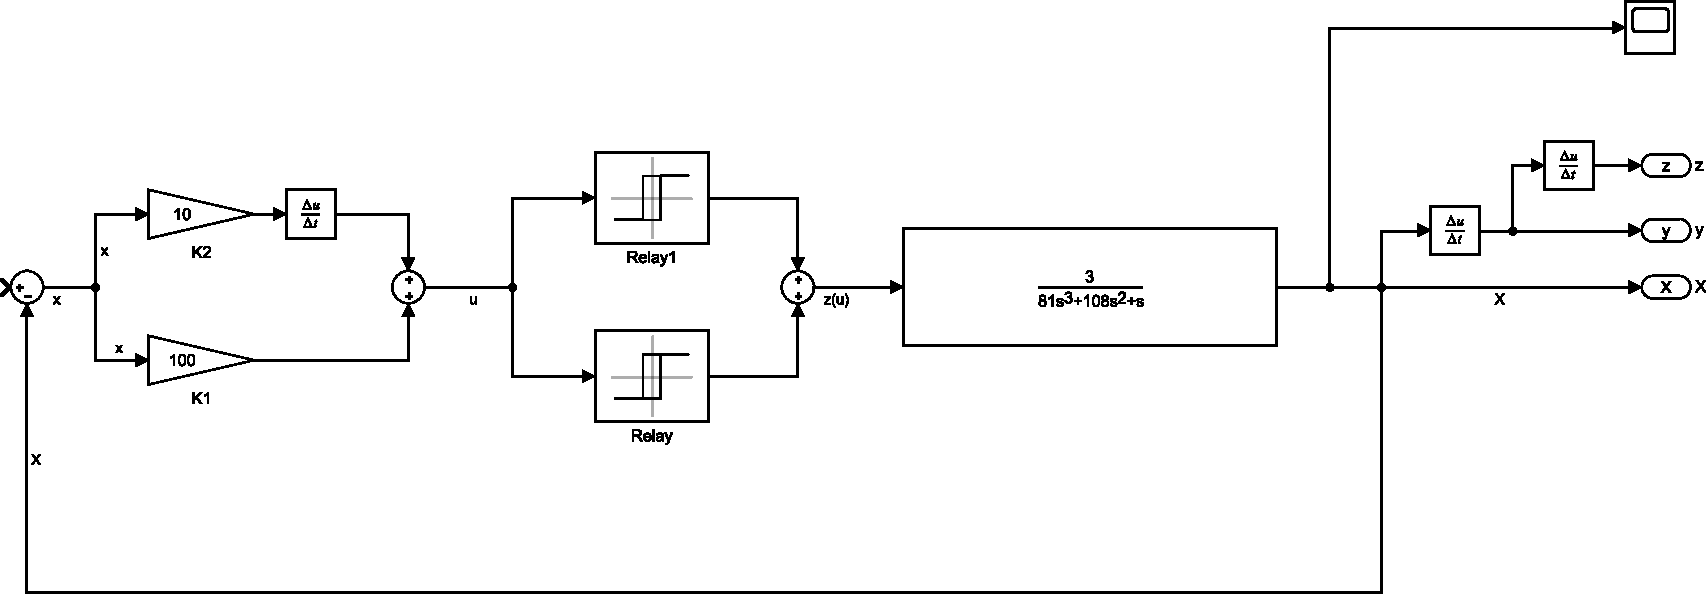
\includegraphics[width=1.0\linewidth]{images/sim_relay_system}
\caption{Структурная схема релейной системы управления с обратной связью.}\label{fig:sim_relay_system}
\end{figure}

Система состоит из линейной части, релейного элемента и пропорционально-дифференциального регулятора. Как будет показано ниже, структура и параметры регулятора существенным образом влияют свойства релейной системы, в том числе и на устойчивость, что необходимо при построении нелинейных систем с переменной структурой.

Чтобы получить трехпозиционное реле без гистерезиса, собираем схему из суммы двух релейных звеньев (двухпозиционное реле с гистерезисом) и настраиваем релейные элементы (Relay) следующим образом:
\begin{equation}
    \begin{aligned} \label{eq:}
       &\text{Relay} & &\text{Relay1}\\
       &\text{Switch on point: } 0.6 &&\text{Switch on point: } -0.6\\
       &\text{Switch off point: } 0.6 &&\text{Switch off point: } -0.6\\
       &\text{Switch when on: } 0.6 &&\text{Switch when on: } 0\\
       &\text{Switch when off: } 0 &&\text{Switch when off: } -0.6\\
    \end{aligned}
\end{equation}

Определим с помощью моделирования параметры пропорционально- дифференциального регулятора, которые обеспечат существование автоколебательного режима. Например, при $k_1=100$ и $k_2=10$  в релейной системе получим автоколебания.

Исследуем движение фазовых координат во времени посредством моделирования процессов в системе при отклонении системы от состояния равновесия. Фазовые траектории в системе на рис.\ref{fig:relay_system_ft_relay_2}. 
В дополнение на рис.\ref{fig:relay_system_sv_relay} указано изменение выходной переменной и её производной. 
\begin{figure}[!h]\centering
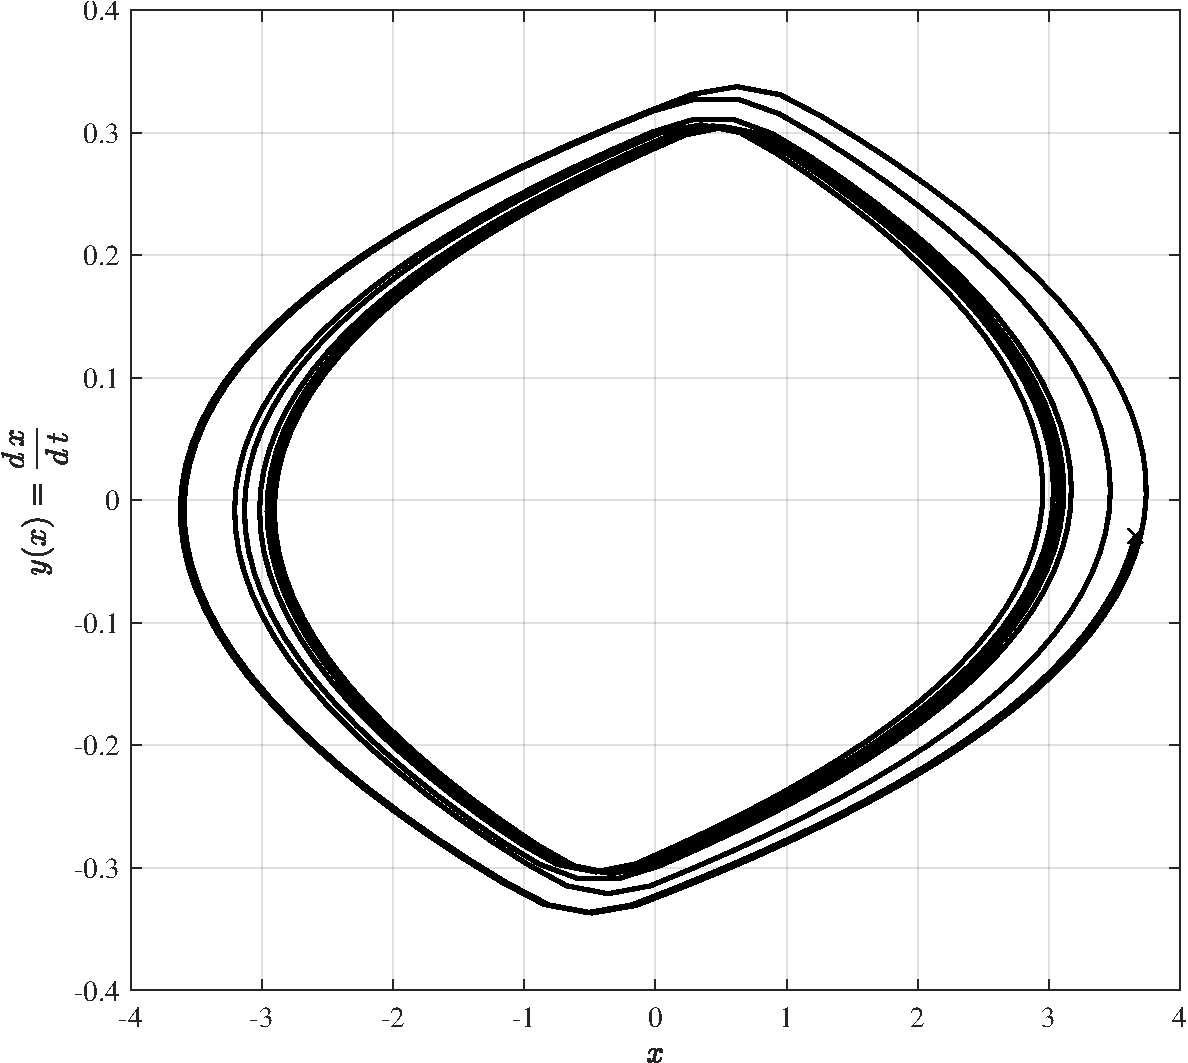
\includegraphics[width=0.7\linewidth]{images/relay_system_ft_relay_2}
\caption{ Фазовые траектории для системы  для переменных состояния $x_1,x_2$.}\label{fig:relay_system_ft_relay_2}
\end{figure}
\begin{figure}[!h]\centering
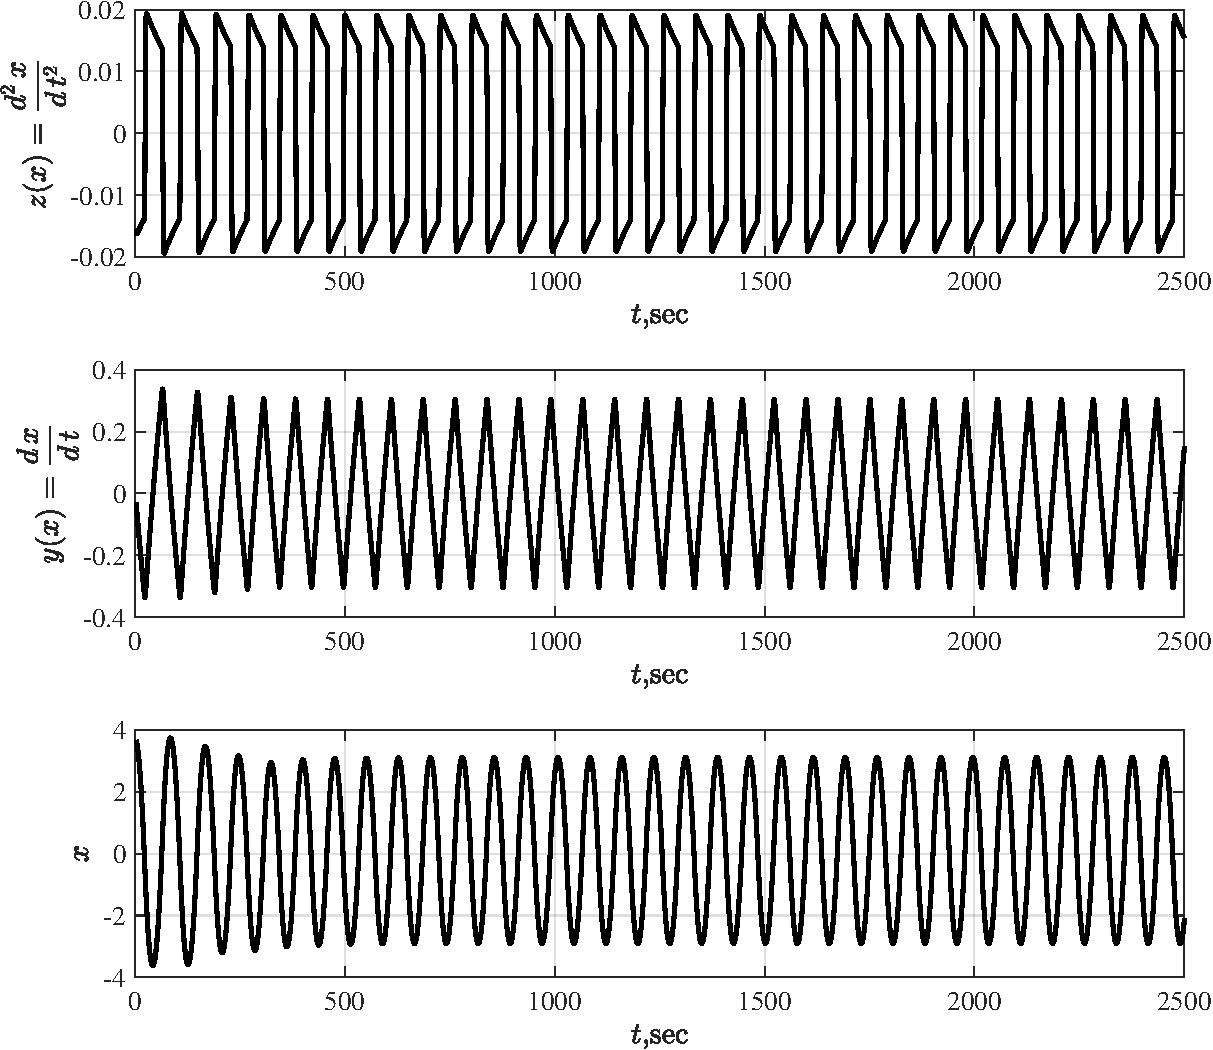
\includegraphics[width=1.0\linewidth]{images/relay_system_sv_relay}
\caption{ Графики изменения переменных состояния.}\label{fig:relay_system_sv_relay}
\end{figure}


Определим амплитуду и частоту автоколебаний методом гармонической линеаризации и гармонического баланса.

Для нахождения решений данного уравнения чаще всего применяют аналитические или графоаналитические методы. Воспользуемся графоаналитическим методом нахождения решений уравнения гармонического баланса. Для этого построим на комплексной плоскости два графика: $W_НЭ$ (A) и $\cfrac{-1}{W(j\,w)}$. Найдем точку их пересечения, координаты которой дадут амплитуду и частоту автоколебаний.
Коэффициент гармонической линеаризации для трехпозиционного реле имеет вид:
\begin{equation} \label{eq:}
W_{ne}(A)=\cfrac{4}{\pi\cdot A}\cdot\sqrt{1-\cfrac{\Delta^2}{A^2}}\text{, при }A\ge\Delta
\end{equation}
где $\Delta=d$ – параметр, определяющий зону нечувствительности реле; $A$ – амплитуда возможных колебаний.
\begin{equation} \label{eq:}
W=\cfrac{3\,(k_1+k_2\,p)}{p\,\left(81\,p^2+108\,p+1\right)}
\end{equation}
\begin{equation} \label{eq:}
-\cfrac{1}{W(p)}=-\cfrac{81\,p^3+108\,p^2+p}{30\,p+300}
\end{equation}
\begin{equation} \label{eq:}
-\cfrac{1}{W(j*w)}=\cfrac{w^3\,81{}\mathrm{i}+108\,w^2-w\,1{}\mathrm{i}}{300+w\,30{}\mathrm{i}}
\end{equation}
\begin{equation} \label{eq:}
-\cfrac{1}{W(j*w)}=\cfrac{w^2\,\left(81\,w^2+1079\right)}{30\,\left(w^2+100\right)}+\cfrac{w\,\left(351\,w^2-5\right)}{15\,\left(w^2+100\right)}\,j
\end{equation}

Программа построения графиков и для нахождения решения уравнения в среде Matlab имеет вид:
\begin{verbatim}
%% вывод ХП 
syms p w real;
u= k(1) + k(2)*p ;
den=(T^2*p^3+2*h*T*p^2+p) ;
W=K*u/den;
W1=-1/W
W1=subs(W1,p,1i*w)
re=simplify(real(W1))
im=simplify(imag(W1))
%% solve
syms w ;
assume(w > 0);
w = double(solve(im,w))
syms A;
Wne=4/(pi*A)*(sqrt(1-(d/A)^2));
A = double(solve(Wne-double(subs(re,'w',w)),A))
%% graphic
step=w/100;
wz=0:step:w;
rele=double(subs(re,'w',wz));
imle=double(subs(im,'w',wz));

hold on,grid on
plot(rele,imle);
xlabel('Re'),ylabel('Im')

step=(min(A)-d)/100;
Az=d:step:min(A)+step;
rene=double(subs(Wne,'A',Az));
imne=zeros(length(rene));
plot(rene,imne);
\end{verbatim}
\begin{figure}[!h]\centering
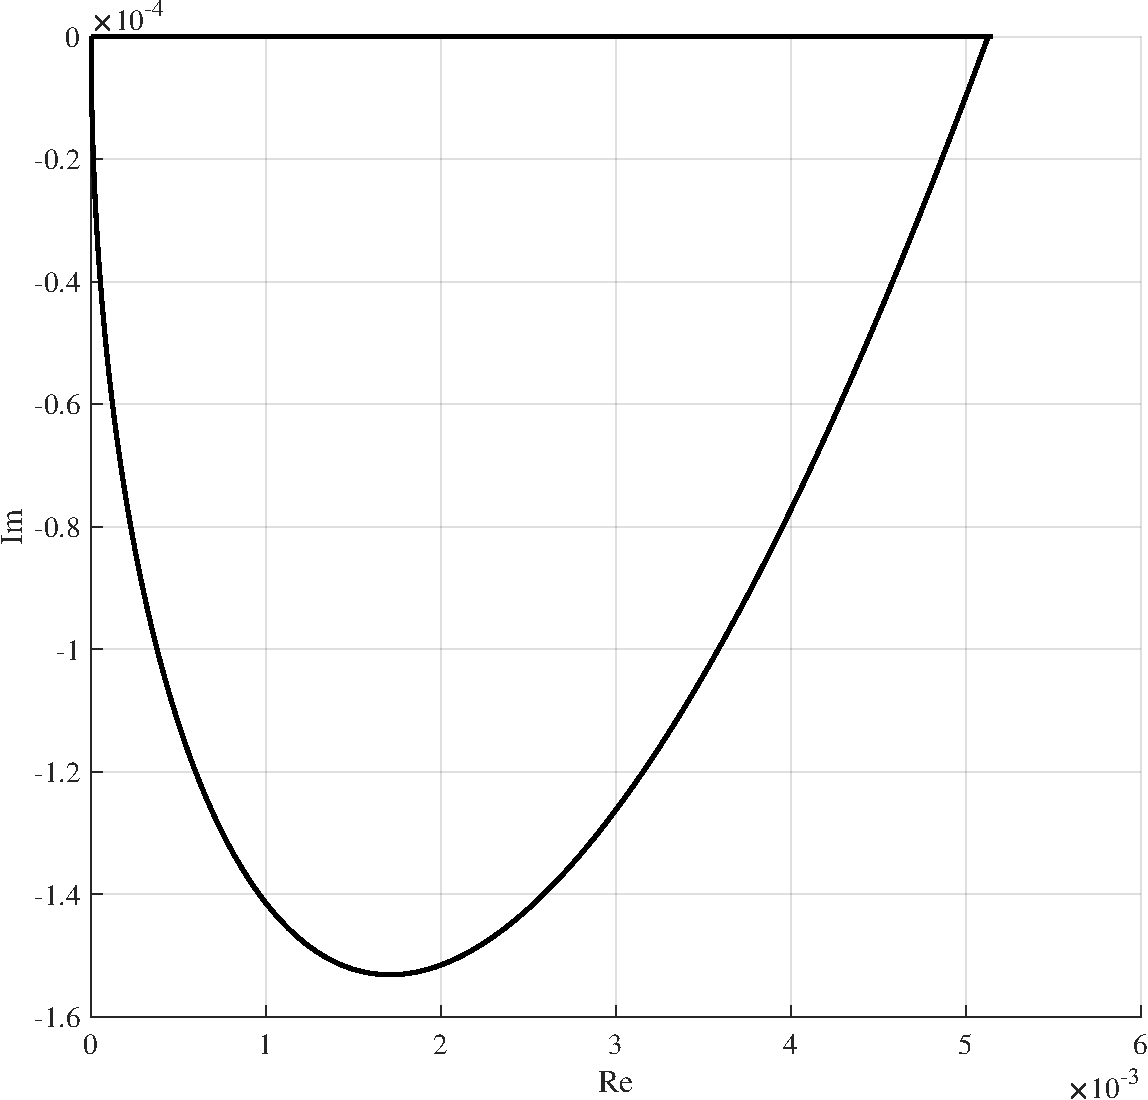
\includegraphics[width=0.6\linewidth]{images/relay_find_param}
\caption{ . Определение параметров автоколебательного режима методом гармонического баланса.}\label{fig:relay_find_param}
\end{figure}

Частота автоколебаний получилась $w_{ak}=0.119$, амплитуда получилась $A_{ak}=248$.
В результате синтеза для рассматриваемого случая уравнение линии переключения получится в виде: $S_2=100\,x_1+10\,x_2+d_{s}$.
